\documentclass[tikz]{standalone}

\usepackage{tikz}
\usetikzlibrary{decorations}
\usetikzlibrary{decorations.pathreplacing, intersections}
\usepackage{pgfplots}
\usetikzlibrary{calc,positioning}
\pgfplotsset{compat=newest, scale only axis, width = 10cm}

% ---------------------------------------------------------------------
% Coordinate extraction
% #1: node name
% #2: output macro name: x coordinate
% #3: output macro name: y coordinate
\newcommand{\Getxycoords}[3]{%
    \pgfplotsextra{%
        % using `\pgfplotspointgetcoordinates' stores the (axis)
        % coordinates in `data point' which then can be called by
        % `\pgfkeysvalueof' or `\pgfkeysgetvalue'
        \pgfplotspointgetcoordinates{(#1)}%
        % `\global' (a TeX macro and not a TikZ/PGFPlots one) allows to
        % store the values globally
         \global\pgfkeysgetvalue{/data point/x}{#2}%
         \global\pgfkeysgetvalue{/data point/y}{#3}%
     }%
}
% ---------------------------------------------------------------------

% Create fake \onslide and other commands for standalone picture
\usepackage{xparse}
\NewDocumentCommand{\onslide}{s t+ d<>}{}
\NewDocumentCommand{\only}{d<>}{}
\NewDocumentCommand{\uncover}{d<>}{}
\NewDocumentCommand{\visible}{d<>}{}
\NewDocumentCommand{\invisible}{d<>}{}

% \pgfplotsset{
%     onslide/.code args={<#1>#2}{% http://tex.stackexchange.com/a/6155/16595
%         \only<#1>{\pgfkeysalso{#2}}
%     },
%     alt/.code args={<#1>#2#3}{%
%         \alt<#1>{\pgfkeysalso{#2}}{\pgfkeysalso{#3}} % \pgfkeysalso doesn't change the path
%     },
% }

\begin{document}

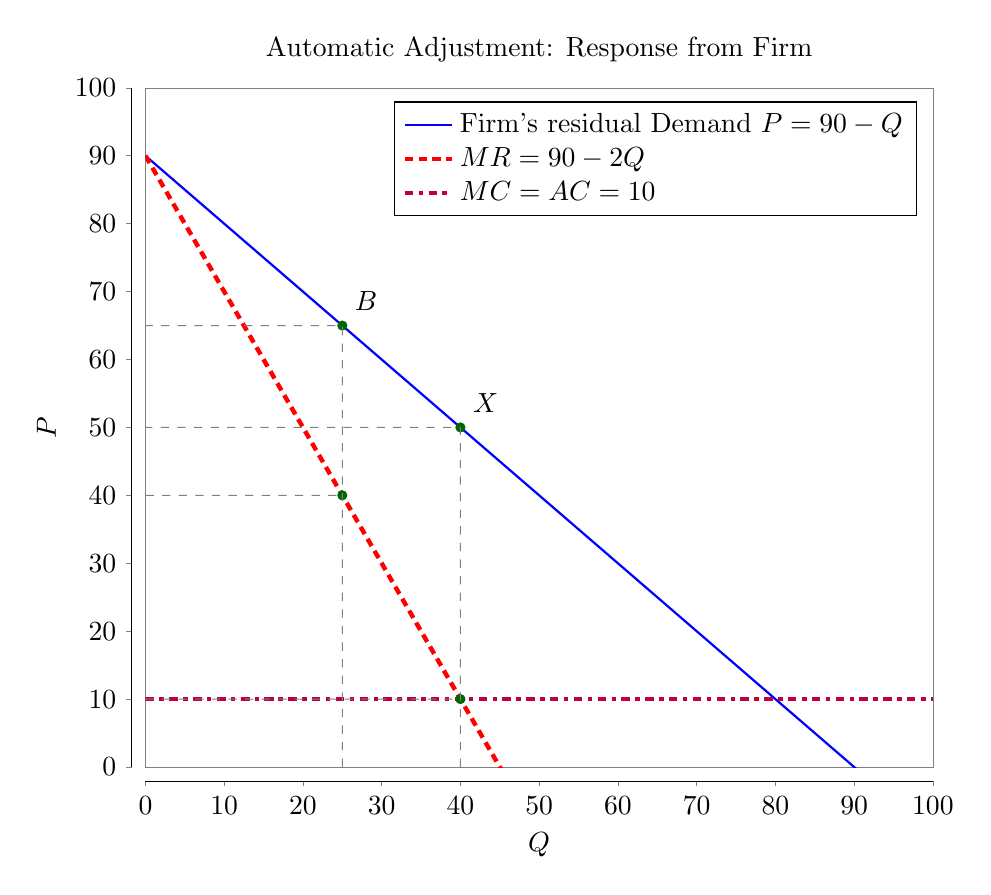
\begin{tikzpicture}

\begin{axis}[
    xmin = 0,
    xmax = 100,
    ymin = 0,
    ymax = 100,
    xlabel = {$Q$},
    ylabel = {$P$},
    sciclean/.style={axis lines=left,
        axis x line shift=0.5em,
        axis y line shift=0.5em,
        axis line style={-,very thin},
        axis background/.style={draw,ultra thin,gray},
        tick align=outside,
        major tick length=2pt},
    xtick distance=10,
    ytick distance=10,
    title = {Automatic Adjustment: Response from Firm},
    domain = 0:100,
    legend cell align = left,
    % legend pos = outer north east,
    sciclean]

    \addplot[name path = D, thick, color = blue, samples = 100] {90 - x};
    \addlegendentry{Firm's residual Demand $P = 90 -Q $}
    % \addplot[name path = R, thick, color = pink, dashed, samples = 100] {(90 - 5*x)*x};
    % \addlegendentry{$R = P(Q) \times  Q$}
    \addplot[name path = MR, ultra thick, color = red, densely dashed, samples = 100] {90 - 2*x};
    \addlegendentry{$MR = 90 - 2Q$}
    % \addplot[name path = C, thick, color = blue, densely dotted, samples = 100] {x^1.8 + 30};
    % \addlegendentry{$ C(Q) = Q^{1.8} + 30$}
    \addplot[name path = MC, ultra thick, color = purple, dashdotted, samples = 100] {10};
    \addlegendentry{$ MC = AC  = 10 $}

    \addplot[name path = MCB, draw = none, ultra thick,  color = orange, dashdotted, samples = 100] {40};
    % \addlegendentry{$ MC = AC  = 40 $}

    \path[name intersections={of = MC and MR, by=MRMC}];
    \node[fill=black!60!green,circle,inner sep=1.3pt, label={[align=left] }] at (MRMC)  {};
    \Getxycoords{MRMC}{\xRC}{\yRC}
    \draw[dashed, gray] (0, \yRC) -- (MRMC);

    \path[name path = xRC] (\xRC, 0) -- (\xRC, 100);
    \path[name intersections={of = D and xRC, by=DxRC}];
    \node[fill=black!60!green,circle,inner sep=1.3pt, label={[align=left] 60:$X$ }] at (DxRC)  {};
    \Getxycoords{DxRC}{\DxRC}{\DyRC}
    \draw[dashed, gray] (\xRC, 0) -- (DxRC) -- (0, \DyRC);

    \path[name intersections={of = MCB and MR, by=MRMC}];
    \node[fill=black!60!green,circle,inner sep=1.3pt, label={[align=left] }] at (MRMC)  {};
    \Getxycoords{MRMC}{\xRC}{\yRC}
    \draw[dashed, gray] (0, \yRC) -- (MRMC);

    \path[name path = xRC] (\xRC, 0) -- (\xRC, 100);
    \path[name intersections={of = D and xRC, by=DxRC}];
    \node[fill=black!60!green,circle,inner sep=1.3pt, label={[align=left] 60:$B$ }] at (DxRC)  {};
    \Getxycoords{DxRC}{\DxRC}{\DyRC}
    \draw[dashed, gray] (\xRC, 0) -- (DxRC) -- (0, \DyRC);



\end{axis}


\end{tikzpicture}

\end{document}
